\documentclass{ximera}

% Mi trad� quell'alma ingrata, infelice, o Dio, mi fa

\usepackage{todonotes}

\newcommand{\RR}{\mathbb R}
\renewcommand{\d}{\,d}
\newcommand{\dd}[2][]{\frac{d #1}{d #2}}
\renewcommand{\l}{\ell}
\newcommand{\ddx}{\frac{d}{dx}}
\newcommand{\dfn}{\textbf}
\newcommand{\eval}[1]{\bigg[ #1 \bigg]}
\renewcommand{\epsilon}{\varepsilon}
\newcommand{\p}[1]{\left(#1\right)}
\newcommand{\br}[1]{\left[#1\right]}
\newcommand{\set}[1]{\left\{#1\right\}}


\let\prelim\lim
\renewcommand{\lim}{\displaystyle\prelim}

\colorlet{textColor}{black} 
\colorlet{background}{white}
\colorlet{penColor}{blue!50!black} % Color of a curve in a plot
\colorlet{penColor2}{red!50!black}% Color of a curve in a plot
\colorlet{penColor3}{red!50!blue} % Color of a curve in a plot
\colorlet{penColor4}{green!50!black} % Color of a curve in a plot
\colorlet{penColor5}{orange!80!black} % Color of a curve in a plot
\colorlet{fill1}{blue!50!black!20} % Color of fill in a plot
\colorlet{fill2}{blue!10} % Color of fill in a plot
\colorlet{fillp}{fill1} % Color of positive area
\colorlet{filln}{red!50!black!20} % Color of negative area
\colorlet{gridColor}{gray!50} % Color of grid in a plot


\newcommand{\fullwidth}{}
\newcommand{\normalwidth}{}



%% makes a snazzy t-chart for evaluating functions
\newenvironment{tchart}{\rowcolors{2}{}{background!90!textColor}\array}{\endarray}


\author{Gregory Hartman \and Matthew Carr}
\license{Creative Commons 3.0 By-NC}
\acknowledgement{https://github.com/APEXCalculus}


\begin{document}

\begin{exercise}

\outcome{Use limit laws.}
\outcome{Calculate limits of the form $0/0$}

  Find 
  \[
  \displaystyle \lim_{x\to3} \frac{x^2-2x-3}{x^2-4x+3}
  \begin{prompt}
  = \answer{2}.
  \end{prompt}
  \]
    \begin{hint}
      This function is \underline{not} continuous everywhere, but both the numerator and denominator are continuous everywhere as functions. Thus, if the limit of $\frac{x^2-2x-3}{x^2-4x+3}$ as $x\to{a}$ does not exist, then the denominator $x^2-4x+3$ must be zero at $a$. Does $x^2-4x+3=0$ when $x=3$? Does $x^2-2x-3=0$ at $x=3$ as well?
    \end{hint}
     \begin{hint}
    Take a look at the graph of the function
    \begin{center}
     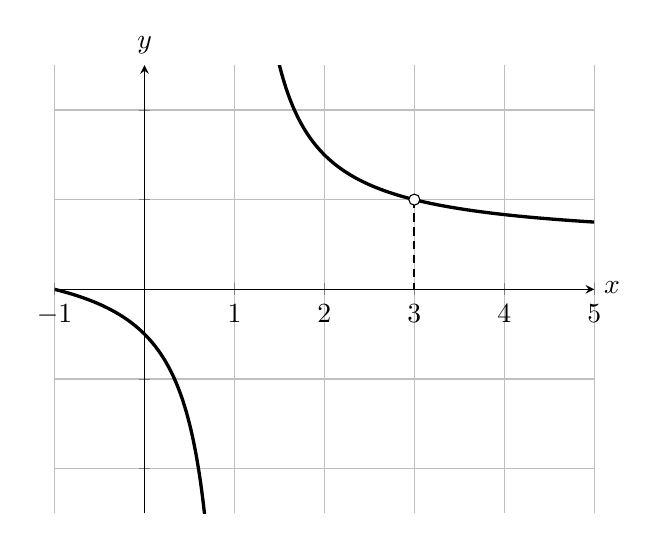
\begin{tikzpicture}
	\begin{axis}
	[ymin=-5,ymax=5, axis lines=center,xlabel=$x$,ylabel=$y$,every axis y 
	label/.style={at=(current axis.above origin),anchor=south},every axis x label/.style={at=(current axis.right of origin),anchor=west},
	domain=-1:5,
	yticklabels={},
	ymajorgrids=true,
	grid = major
	]
	\addplot[domain=-1:99/100,very thick,smooth,samples=500]
	{(\x^2-2*\x-3)/(\x^2-4*\x+3)};
	\addplot[domain=101/100:5,very thick,smooth,samples=500]
	{(\x^2-2*\x-3)/(\x^2-4*\x+3)};
	\draw[densely dashed, thick] (axis cs:3,2)--(axis cs:3,0);
	\draw[fill=white] (axis cs:3,2) circle [radius=2pt];
	\end{axis}
       \end{tikzpicture}      
      \end{center}
      There is a removable discontinuity at $x=3$. This suggests something about the factorization of both polynomials $x^2-2x-3$ and $x^2-4x+3$. Recall that $\lim\limits_{x\to a}\frac{f(x)}{g(x)}=\frac{\lim\limits_{x\to a}f(x)}{\lim\limits_{x\to a}g(x)}$ if $g(a)\ne0$ and both $f(x)$ and $g(x)$ are continuous at $a$.
    \end{hint}
    \begin{hint}
     Notice that the quadratic equation tells us that $x^2-2x-3=0$ has solutions $1\pm2$ and $x^2-4x+3=0$ has solutions $2\pm{1}$. Thus, $x^2-2x-3=\left(x-3\right)\left(x+1\right)$ and $x^2-4x+3=\left(x-3\right)\left(x-1\right)$. Then for any number $a\ne3$, applying the limit law relating quotients of functions,  $\lim\limits_{x\to a}\frac{x^2-2x-3}{x^2-4x+3}=\frac{\lim\limits_{x\to a}\p{x+1}}{\lim\limits_{x\to a}\p{x-1}}$. 
    \end{hint}
\end{exercise}

\end{document}